\documentclass[tikz,border=5mm]{standalone}
\usepackage[T1]{fontenc}
\usepackage{helvet}
\renewcommand{\familydefault}{\sfdefault}
\usetikzlibrary{arrows.meta,positioning,fit,backgrounds,shapes.geometric}

\begin{document}
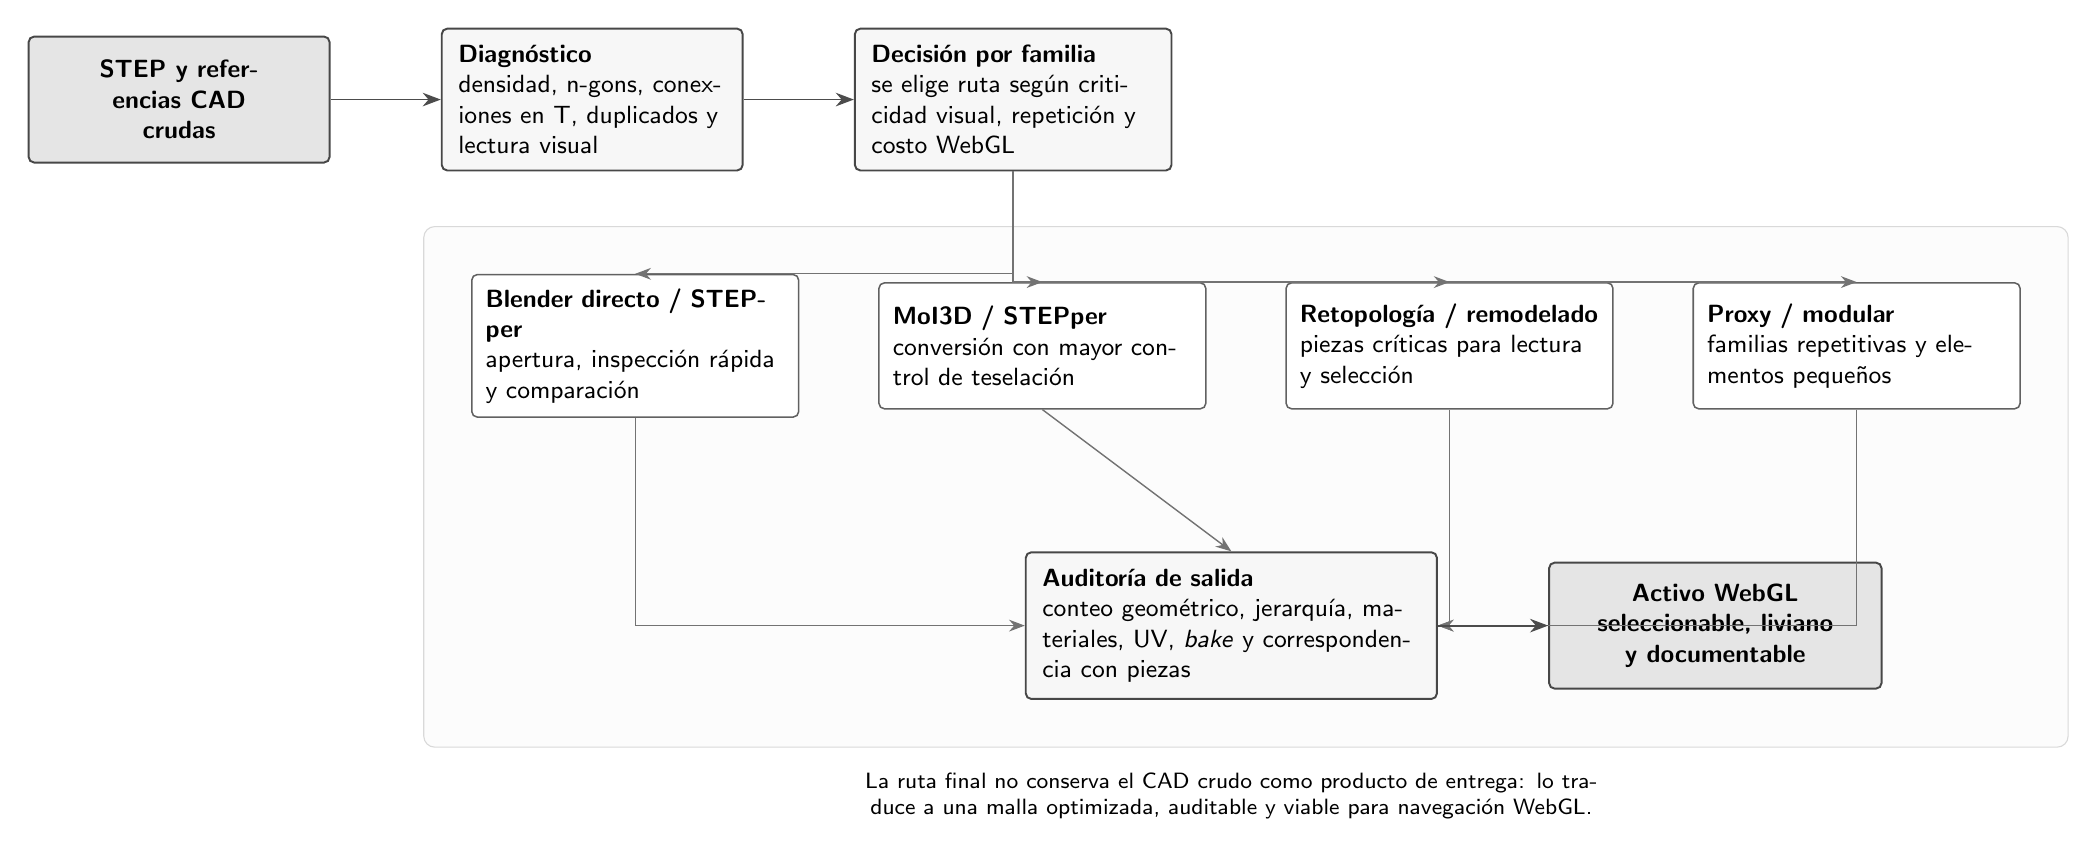
\begin{tikzpicture}[
  font=\sffamily\small,
  node distance=10mm and 14mm,
  box/.style={
    draw=black!72,
    rounded corners=2pt,
    line width=0.7pt,
    fill=black!3,
    align=left,
    text width=34mm,
    inner sep=6pt,
    minimum height=16mm
  },
  head/.style={
    box,
    fill=black!10,
    font=\sffamily\bfseries\small,
    align=center
  },
  route/.style={
    draw=black!62,
    rounded corners=2pt,
    line width=0.55pt,
    fill=white,
    align=left,
    text width=38mm,
    inner sep=5pt,
    minimum height=16mm
  },
  arrow/.style={-{Stealth[length=2.3mm]}, line width=0.65pt, draw=black!70},
  thin/.style={-{Stealth[length=2mm]}, line width=0.5pt, draw=black!55}
]

\node[head] (cad) {STEP y referencias CAD\\crudas};
\node[box, right=of cad] (diag) {\textbf{Diagn\'ostico}\\densidad, n-gons, conexiones en T, duplicados y lectura visual};
\node[box, right=of diag, text width=36mm] (decision) {\textbf{Decisi\'on por familia}\\se elige ruta seg\'un criticidad visual, repetici\'on y costo WebGL};

\node[route, below=13mm of decision, xshift=-48mm] (directa) {\textbf{Blender directo / STEPper}\\apertura, inspecci\'on r\'apida y comparaci\'on};
\node[route, right=10mm of directa] (control) {\textbf{MoI3D / STEPper}\\conversi\'on con mayor control de teselaci\'on};
\node[route, right=10mm of control] (retopo) {\textbf{Retopolog\'ia / remodelado}\\piezas cr\'iticas para lectura y selecci\'on};
\node[route, right=10mm of retopo] (proxy) {\textbf{Proxy / modular}\\familias repetitivas y elementos peque\~nos};

\node[box, below=18mm of control, xshift=24mm, text width=48mm] (audit) {\textbf{Auditor\'ia de salida}\\conteo geom\'etrico, jerarqu\'ia, materiales, UV, \textit{bake} y correspondencia con piezas};
\node[head, right=14mm of audit, text width=38mm] (unity) {Activo WebGL\\seleccionable, liviano y documentable};

\draw[arrow] (cad) -- (diag);
\draw[arrow] (diag) -- (decision);

\draw[thin] (decision.south) |- (directa.north);
\draw[thin] (decision.south) |- (control.north);
\draw[thin] (decision.south) |- (retopo.north);
\draw[thin] (decision.south) |- (proxy.north);

\draw[thin] (directa.south) |- (audit.west);
\draw[thin] (control.south) -- (audit.north);
\draw[thin] (retopo.south) |- (audit.east);
\draw[thin] (proxy.south) |- (audit.east);
\draw[arrow] (audit) -- (unity);

\begin{scope}[on background layer]
  \node[draw=black!15, rounded corners=4pt, fill=black!1,
    fit=(directa)(proxy)(audit),
    inner sep=6mm] {};
\end{scope}

\node[align=center, font=\sffamily\footnotesize, text width=118mm,
  below=8mm of audit] (note)
  {La ruta final no conserva el CAD crudo como producto de entrega: lo traduce a una malla optimizada, auditable y viable para navegaci\'on WebGL.};

\end{tikzpicture}
\end{document}
